\documentclass{article}
\usepackage[utf8]{inputenc}
\textheight = 25cm 
\textwidth = 15cm
\topmargin = -3.0cm 
\oddsidemargin = 1.5cm
\usepackage{hyperref}
\hypersetup{
    colorlinks=true,
    linkcolor=blue,
    filecolor=blue,
    citecolor=black,      
    urlcolor=blue,
    }

\usepackage{float}
\usepackage{graphicx}

\usepackage{gensymb}

\usepackage{amsmath}
\usepackage{amssymb}
\usepackage{amsfonts}
\usepackage{mathtools, xparse}
\usepackage[shortlabels]{enumitem}

\usepackage[many]{tcolorbox}
\usepackage{lipsum}
\usepackage{amssymb}

\title{Tarea 1 Termodinámica}
\author{Cerritos Lira, Carlos\\
Calderón Alba, Sebastián \\ Pérez Anaya, Gustavo Miguel\\ 
Velasco Salazar, Pablo}
\date{3 de abril del 2020}

\newcommand{\pr}[1]{\left(#1\right)}
\newcommand{\pt}[2]{\dfrac{\partial #1}{\partial #2}}

\begin{document}
\maketitle
\section*{1.-}
Las isotermas de un sistema pueden cortarse? Explique detalladamente.
\begin{tcolorbox}[breakable]
    \subsubsection*{Caso general}
    Dado un sistema  y su funcion de estado 
    \[ f(P,V,T) = 0 \]
    es verdad que dado $(P_0,V_0,T_0)$, podemos obtener localmente una función 
    $T(P,V)$ tal que:
    \[ f(P,V,T(V,P)) = 0 \quad \forall (P,V) \in B_{\delta}(P_0,V_0) \] 
    las isotermas no se pueden cruzar si esta función local se puede 
    hacer global, sin embargo este no es siempre el caso.
    \subsubsection*{Gas ideal}
    En este modelo:
    \begin{align*}
        PV &= nRT \\
        T(V,P) &= \frac{PV_m}{R}   
    \end{align*}
    claramente pudimos obtener $T$ de forma global entonces las isotermas no se intersectan.

    \subsubsection*{Redlich–Kwong}  
    En este modelo:
    \begin{align*}
        P = \frac{RT}{V_m-b} - \frac{a}{\sqrt{T}V_m(V_m+b)}
    \end{align*}
    se puede demostrar que no hay una función que cumpla:
    \begin{align*}
        f(P,V,T(P,V)) &= 0 \quad \forall (V,P)
    \end{align*}
    se puede entonces tener dos temperaturas para el mismo volumen y presión. 
\end{tcolorbox}

\section*{2.-}
Sean $A,B,C$ tres gases con variables $(p,V),(p',V'),(p'',V'')$, respectivamente. 
Cuando $A$ está en equilibrio térmico con $C$ se satisface la ecuación:
\begin{align*}
    pV - nbp - p''V'' = 0
\end{align*}
cuando $B$ está en equilibrio térmico con $C$ se cumple:
\begin{align*}
    p'V' - p''V'' + \frac{nB'p''V''}{V'} &= 0
\end{align*}
\begin{enumerate}[a)]
    \item Encuentre las funciones $q(p,V),r(p',V')$ y $s(p'',V'')$ que son iguales 
    entre si en el equilibrio térmico e iguales a la temperatura común $T$.

    \item Encuentre la ecuación que corresponde a $A$ en equilibrio térmico con $B$
\end{enumerate}

\begin{tcolorbox}[breakable]
    \subsection*{a)} Recrodemos que para que se cumpla la Ley Cero se debe cumplir 
    
    \begin{align*}
        F_{ac}&=g\pr{V_c}h\pr{p_a,V_a}+J\pr{V_c}\\
        F_{bc}&=g\pr{V_c}h\pr{p_b,V_b}+J\pr{V_c}
    \end{align*}
    
    donde $F_{ac}$ y $F_{bc}$ hacen referencia al equilibrio termodinpamico entre los sistemas $AC$ y $BC$. Veamos que para que $F_{ac}=F_{bc}$ se debe cumplir que $h\pr{p_a,V_a}=h\pr{p_b,V_b}$. En este caso tendemos que del sistema $AC$
    
    \begin{align*}
        pV-nbp-p''V''&=0\\
        \Rightarrow p''V''&=pV-nbp
    \end{align*}
    
    Por otra parte, del sistema $BC$ tenemos que
    
    \begin{align*}
        p'V'-p''V''+\dfrac{nB'p''V''}{V'}&=0\\
        \Rightarrow p''V''\pr{-1+\dfrac{nB'}{V'}}&=-p'V'\\
        \Rightarrow p''V''\pr{nB'-V'}&=-pV'^2\\
        \Rightarrow p''V''&=\dfrac{pV'^2}{V'-nB'}
    \end{align*}
    
    De igualar las ecuaciones anteriores es facil ver la siguiente igualdad
    
    \begin{align*}
        pV-nbp=\dfrac{p'V'^2}{V'-nB'}=p''V''
    \end{align*}
    
    donde todas son iguales a la temperatura común, eotnces podemos fer que las funciones que buscábamos
    
    \begin{align*}
        q&\pr{p,V}=pV-nbp\\
        r&\pr{p',V'}=\dfrac{p'V'^2}{V'-nB'}\\
        s&\pr{p'',V''}=p''V''
    \end{align*}
    
    
    
    \subsection*{b)}
    Para hallar esta ecuación despejaremos $p''V''$ de las dos ecuaciones de equilibrio dadas en el problemas, es decir 
    
    \begin{align*}
        p''V''=pV-nbp \tag{2.1}
    \end{align*}
    
    Por otro lado 
    
    \begin{align*}
        p''V''\left(-1+\dfrac{nB'}{V'}\right)&=-p'V'\\
        \Rightarrow p''V''\left(nB'-V'\right)&=-pV'^2\\
        \Rightarrow p''V''&=\dfrac{pV'^2}{V'-nB'} \tag{2.2}
    \end{align*}
    
    Ahora, igualamos \textbf{(2.1)} con \textbf{(2.2)}
    
    \begin{align*}
        \Rightarrow pV-nbp=\dfrac{pV'^2}{V'-nB'}\\
        \therefore pV+\dfrac{pV'^2}{nB'-V'}-nbp=0
    \end{align*}
    
    Ésta es la ecuación que corresponde a $A$ en equilibrio térmico con $B$
    
    
\end{tcolorbox}
\section*{3.-}
Un gas ideal se caracteriza mediante dos suposiciones: los átomos o moléculas de un gas 
ideal no interactúan entre sí, y los átomos o moléculas se pueden tratar como masas 
puntuales. Esto tiene un rango de validez limitada. \\ \\ 
Se muestra la energía potencial de interacción de dos moléculas de gas en función 
de la distancia entre ellas. El potencial intermolecular se peude dividir en regiones
en las que la energía potencial es esencialmente nula $(r>r_{trans})$, negativa
(interacción atractiva) $(r_{trans} > r > r_{V=0})$, y positiva (interacción repulsiva).
La distancia $r_{trans}$ no está defininida unívocamente y depende de la energía de la 
molécula.

\begin{enumerate}[a)]
    \item Calcule la presión ejercida por $N_2$ a $300K$ para vólumenes molares de 
    $250$ y $0.100L$ usando las ecuaciones de estado del gas ideal y de van der Waals.
    Los valores de los parámetros $a$ y $b$ para $N_2$ son $1.360bar dm^3 mol^{-2}$ y
    $0.0387 dm^3 mol^{-1}$ respectivamente. 
    
    \item Compare y explique los reusltados de los cálculos a las dos presiones y 
    explique qué predomina, las intersacciones atractivas o las repulsivas.

    \item A temperatura suficientemente elevada, la ecuación de van der Waals tiene 
    la forma $P = \frac{RT}{V-b}$. Nótese que la parte atractiva del potencial no tiene 
    influencia en esta expresión. Justifique este comportamiento uisando el diagrama 
    anterior.
\end{enumerate}

\begin{tcolorbox}[breakable]
    \subsection*{a)}
    De acuerdo al gas ideal:
    \begin{align*}
        P_{I} 
        &= \frac{RT}{V_m} \\
        P_{I_{250}}
        &= RT \cdot 0.004 = 0.09977 bar\\ 
        P_{I_{0.1}}
        &= RT \cdot 10 = 249.43 bar 
    \end{align*}
    De acuerdo a Van der Waals:
    \begin{align*}
        P_{W}
        &= \frac{RT}{(V_m - b)} - \frac{a}{V_m^2} \\
        P_{W_{250}}
        &= RT \cdot 0.004 - 2.17\times 10^{-5} = 0.09976 bar \\
        P_{W_{0.01}}
        &= RT \cdot 16 - 135.99 = 270.905 bar 
    \end{align*}

    \subsection*{b)}
    Podemos ver que se cumplen las relaciones:
    \begin{align*}
        P_{I_{250}} \approx P_{W_{250}} \\
        P_{I_{0.1}} < P_{W_{0.1}}
    \end{align*}
    De acuerdo a la gráfica las interacciones para $V=250L$ nos encontramos en 
    la región $r > r_{trans}$ y para $V=0.1L$ en la región $r < r_V$

    \subsection*{c)}
    De acuerdo a la gráfica de la energía potencial nos encontramos en la región 
    $r > r_{trans}$, esto tiene sentido pues a medida que aumenta el volumen 
    la distancia entre las molélculas del gas es más grande, lo que se ve reflejado  
    en la ecuaciones dado que podemos omitir el término $\frac{1}{V_m^2}$


\end{tcolorbox}
\section*{4.-}
Sabemos que la ecuación de van der Waals permite hacer una descripción cualitativa 
de la transición líquido- vapor, por lo cual, como se mencionó en clase, el 
valor del parámetro $a$ tiene una relación con el calor de vaporzación del líquido y 
el párametro $b$  con el tamaño de las moléculas. Del artículo de van der Waals haga 
una descripción, en no menos de una cuartilla, de lo que son las fuerzas de 
van der Waals, como se analiza en el punto crítico, el factor de compresibildiad y al 
ensión superficial.

\begin{tcolorbox}[breakable]
    La termodinámica tuvo apogeo en la primera revolución industrial, ahí se puso mucha atención al estudio de los gases. Posteriormente, en el siglo XIX se le dio mas atención debido a los procesos que involucraban petroleo y sus derivados para producir energía. \ 
    
    Ahora la termodinámica es una rama de la física que tiene varias aplicaciones; como el desarrollo de nuevas tecnologías para explorar al espacio.\\ 
    
    \textbf{Fuerzas de Van der Waals}\
    
    Con los trabajos de  Boyle y Gay-Lussac se tenía un estudio de los gases, pero para las necesidades de la época no eran suficientes. Pero fue con Johannes Diderik Van der Waals, quien modifico el modelo previo considerando que las moléculas ocupan cierto espacio, tienen forma esferica y además que ejercen fuerzas atractivas entre ellas.\
    
    En su modelo incluyo dos nuevas constantes, \textit{a} y \textit{b}, donde esta ultima hace referencia al volumen esférico que utilizan las partículas, mientras que \textit{a} hace referencia a las fuerzas de cohesión (o atractiva) que hay entre ellas. A las fuerzas de cohesión se les llama fuerzas de Van der Waals o fuerzas de dipolo. \
    
    Así Johannes Diderik Van der Waals unificó casi todo el conocimiento experimental sobre propiedades de los fluidos existentes hasta en 1870 en una única ecuación.\\ 
    
    \textbf{Punto critico}\
    
    Al momento de investigar el comportamiento de los gases, se dieron cuenta de que a cierta temperatura el menisco que marca la división entre la fase liquida y la de vapor de una sustancia desaparecía y la densidad del líquido y el vapor eran las mismas. Eso ocurría debido a que, cuando se sube la temperatura de un sistema líquido, este se expande; mientras que en un sistema con gas aumenta la presión y por ende la densidad del gas. \ 
    
    A este estado se le conoce como \textit{punto critico}, y se le asocian las variables de temperatura critica, volumen critico y presión critica. El resultado que se obtuvo fue que los valores de las constantes \textit{a} y \textit{b} dejaron de ser valores empíricos. \\
    
    \textbf{Factor de compresibilidad}\
    
    El factor de compresibilidad queda definido como la razón entre el volumen molar de un gas real y un gas ideal. Este es para observar que tan parecido es el gas ideal con el gas real, es decir, la desviación. Para el gas ideal este factor es igual a la constante uno. Por ejemplo en los isótopos del gas de Helio es alrededor de 0.30. \
    
    El factor de compresibilidad representa la cercanía con el modelo ideal y se utiliza para comparar el comportamiento de un gas real con respecto al establecido por la ecuación de los gases ideales. \\ 
    
    \textbf{Tensión superficial}\
    
    Esta se define como el trabajo necesario para transportar moléculas hacia la superficie de un líquido. La tensión superficial se debe a que las fuerzas que afectan a cada molécula son diferentes entre el interior del líquido y la superficie. \ 
    
    Entre mas interacciones intermoleculares existan, el trabajo necesario para trasladar las moléculas del interior del líquido a la superficie es mayor, entonces el valor de la tensión superficial es mayor. \\ 
    
\end{tcolorbox}
\section*{5.-}
Sea un gas en un recipiente cilíndrico de un metro de altura, cuya tapa superior es 
un pistón inicialmente fijo. El gas está en equilibrio a temperatura y presión ambiente
y bajo estas condiciones sabemos que la velocidad de propragación del sonido es 
$c = 340 \frac{m}{seg}$. Supongamso que liberamos al pistón para que pueda moverse 
libremente. Ahora le damos un martillazo al pistón, generando así una situación de
desequilibrio en el gas. También inmediatamente aislamos térmicamente al sistema. 
\begin{enumerate}[a)]
    \item Culcule el tiempo que tarda en saber la parte inferior del gas que ha sido 
    golpeado 

    \item Discuta cualitativamente qué ocurrió con la energía proporcionada por el 
    martillazo. 

    \item ¿Se restaura el equilibrio o queda oscilando?
\end{enumerate}

\begin{tcolorbox}[breakable]
    El problema se ilustra en el siguiente diagrama:
    \begin{figure}[H]
        \centering
        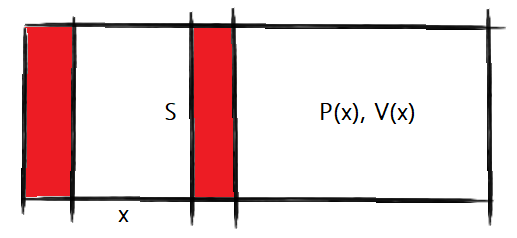
\includegraphics[scale=0.7]{images/p5_piston.png}
        \caption{Diagrama recipiente cilíndrico}
    \end{figure}
    Nuestro objetivo es encontrar la fuerza que actua en el pistón, donde se 
    sabe:
    \begin{align*}
        F &= S(P_0-P)
    \end{align*}
    Como el proceso es adiabático se tiene:
    \begin{align*}
        PV^{\gamma} &= c
    \end{align*}
    sabemos que $V(x) = V_0-Sx$, usando el hecho $\frac{V}{V_0} \in (0,1)$ y
    despejando $P$ obtenemos:
    \begin{align*}
        P &= P_0 \left( \frac{V}{V_0} \right)^{-\gamma} \\ 
        &\approx P_0 \left(-\gamma \left(\frac{V}{V_0}-1\right) + 1\right)  \\
        &\approx P_0 \left(1+\gamma \frac{S}{V_0}x \right)
    \end{align*}
    de donde obtenemos la fuerza:
    \begin{align*}
        F = -\left(P_0\gamma \frac{S}{V_0}\right)x 
    \end{align*}
    Por lo tanto el piston sigue un movimiento armónico simple. 
    \subsection*{a)}
    Para que la onda de presión llege al fondo del recipiente debe de recorrer una 
    distancia de $1-x_0$, de acuerdo a la formula tenemos:
    \begin{align*}
        t 
        &= \frac{d}{V} \\
        &= \frac{1-x_0}{340}[s]
    \end{align*}
    en el caso de que $x_0 \approx 0$ se tiene $t = \frac{1}{340}[s]$
    \subsection*{b)}
    La energía proporcionada es transferida las partículas dentro del cilindro, 
    formandose una onda de presión, esto es $p(x,t)$, la función que nos dice la 
    presión en la posición $x$ al tiempo $t$ satisface la ecuación 
    de onda, con condición inicial $p(x_0,0) = p_0$ donde $p_0$ está dado en 
    función de la energía cinética del martillo durante el golpe, esta onda 
    recorre el cilindro tan rápido que se considera la presión uniforme 
    en todos los puntos. 
    \subsection*{c)}
    Como se vio la fuerza que actua es la del movimiento armónico simple, por lo 
    tanto este es el movimiento que se sigue (si ignoramos la fricción).
    
\end{tcolorbox}
\section*{6.-}
Demuestre que para un gas ideal $pv = RT$, $\beta = \frac{1}{T}$, $k = \frac{1}{p}$. \\
Para un gas real a presiones moderadas, $P(v-b) = RT$, donde $R$ y $b$ son constantes, 
es una ecuación de estado aproximada que tiene en cuenta el tamaño finito de las moléculas.
Demostrar que:
\begin{enumerate}[a)]
    \item $\beta = \frac{\frac{1}{T}}{1+\frac{bP}{RQ}}$
    \item $k = \frac{\frac{1}{p}}{1+\frac{bP}{RT}} $
\end{enumerate}

\begin{tcolorbox}[breakable]
    \subsection*{a)}
    Partiremos de:
    \begin{align*}
        PV &= RT \\
        \beta &= \frac{1}{V}\left(\frac{\partial V}{\partial T}\right)_P \\
         K &= \frac{1}{V}\left(\frac{\partial V}{\partial P}\right)_T
    \end{align*}
    Despejando V:
    \begin{align*}
        V 
        &= \frac{RT}{P}\\
        \frac{\partial V}{\partial T} 
        &= \frac{R}{P} \\
        \frac{\partial V}{ \partial P} 
        &= \frac{-RT}{P^2}   
    \end{align*}
    Sustituyendo en la definición de $\beta, K$:
    \begin{align*}
        \beta 
        &= \frac{1}{V} \frac{R}{P} 
        = \frac{1}{\frac{RT}{P}} \frac{R}{P} 
        = \frac{P}{RT} \frac{R}{P} = \frac{1}{T} \\
        K 
        &= \frac{-1}{V} \left(\frac{-RT}{P^2} \right)
        = \frac{1}{P}
    \end{align*}
    \subsection*{b)}
     Partiremos de:
    \begin{align*}
        P(V-b) &= RT 
    \end{align*}
    Despejando V:
    \begin{align*}
        V 
        &= \frac{RT}{P} + b \\
        \frac{\partial V}{\partial t} 
        &= \frac{R}{P}    \\ 
        \frac{\partial V}{\partial P} 
        &= \frac{-RT}{P^2}    
    \end{align*}
    Sustituyendo en la definición de $\beta$:
    \begin{align*}
        \beta 
        &= \frac{1}{V} \frac{R}{P} \\ 
        &= \frac{1}{\frac{RT}{P}+b} \frac{R}{P} \\  
        &= \frac{RT}{T(RT+Pb)} \\ 
        &= \frac{\frac{1}{V}}{\frac{RT+bP}{RT}} \\
        &= \frac{\frac{1}{T}}{1+\frac{bP}{RT}}
    \end{align*}
    Sustituyendo en la definición de $K$:
    \begin{align*}
        K 
        &= \frac{-1}{V}\left( \frac{-RT}{P^2} \right) \\
        &= \frac{1}{V}\left(\frac{RT}{P^2}\right) \\
        &= \frac{1}{\frac{RT}{P}+b} \left(\frac{RT}{P^2}\right) \\
        &= \frac{P}{RT+Pb} \left(\frac{RT}{P^2}\right) \\
        &=\frac{RT}{(RT+Pb)P}\\
        &= \frac{\frac{1}{P}}{\frac{RT+Pb}{RT}} \\
        &= \frac{\frac{1}{P}}{1+\frac{Pb}{RT}}
    \end{align*}
\end{tcolorbox}


\section*{7.-}
Un hilo metálico de $0.0085cm^3$ de sección transversal está sometido a una tensión de 
$20N$, a la temperatura de $10\degree C$, ente dos soportes rígidos separados $1.2m$. 
\begin{enumerate}[a)]
    \item ¿Cuál es la tensión final, si la temperatura se reduce $8\degree C$?
    $(\alpha = 1.5 \times 10^{-5}K^{-1}), Y = 2.0 \times 10^9 \frac{N}{m^2}$

    \item La frecuencia fundamental de vibración de un alambre de longitud $L$, 
    masa $m$ y tensión $\tau$ es:
    \[ f = \frac{1}{2L} \sqrt{\frac{\tau L}{m}} \]
    ¿Con qué frecuencia vibra el hilo a $20\degree C$. ¿Y a $8\degree C$
\end{enumerate}
\begin{tcolorbox}[breakable]
    \subsubsection*{a)}
    Para este sistema se tiene la relación:
    \begin{align*}
        \frac{\partial \tau}{\partial T} &= -\alpha A Y
    \end{align*}
    integrando obtenemos la tensión en función de T:
    \begin{align*}
        \tau  &= -\alpha A Y (T-10) + \tau_{10} \\ 
        \tau_8 &= 20.0017N
    \end{align*}
    \subsubsection*{b)}
    Como vimos $\tau_8 = 1.00085\tau_{10}$ de donde tenemos:
    \begin{align*}
        f_{10} &= \sqrt{1.00085}f_8\\ 
        f_{10} &= 1.000042f_8 
    \end{align*}
\end{tcolorbox}

\section*{8.-}
Muestre que si las diferenciales $dV, dp$ dadas por:
\begin{align*}
    dV &= V\beta dT - Vk_T dp \\
    dp &= \frac{\beta}{k_T} dT - \frac{1}{k_T}dV
\end{align*}
Son exactas, entonces los coeficientes satisfacen las siguientes relaciones:
\begin{align*}
    \left( \frac{\partial V \beta}{\partial p} \right)_T
    &=-\left( \frac{\partial V_{k_T}}{\partial T} \right)_P \\
     \left( \frac{\partial \beta}{\partial V} \right)_T
    &=\beta \left( \frac{\partial lnK_T}{\partial V} \right) 
    + \frac{1}{V}\left( \frac{\partial lnK_T}{\partial T} \right)
\end{align*}

\begin{tcolorbox}[breakable]
Recordemos que podemos ver la diferencial de $V$ como
\begin{align*}
    dV=\pr{\pt{V}{T}}_PdT+\pr{\pt{V}{P}}_Tdp
\end{align*}

De las relaciones dadas en el problema podemos hacer las siguientes igualdades
\begin{align*}
    \pr{\pt{V}{T}}_P&=V\beta \\
    \pr{\pt{V}{P}}_T&=-Vk_T
\end{align*}

Y como las diferenciales son exactas entonces tenemos que 
\begin{align*}
    \pr{\pt{}{p}\pr{\pt{V}{T}}_p}_T&=\pr{\pt{}{T}\pr{\pt{V}{p}}_T}_p\\
    \Rightarrow \pr{\pt{}{p}V\beta}_T&=\pr{\pt{}{T}-Vk_T}_p\\
    \therefore \pr{\pt{V\beta}{p}}_T&=-\pr{\pt{Vk_t}{T}}_p
\end{align*}

\end{tcolorbox}
\section*{9.-} 
La resistencia eléctrica en el hilo de un termómetro de platino varía linealmente con
la temperatura. Determinar:
\begin{enumerate}
    \item La expresión de la temperatura centígrada en el punto de fusión del hielo 
    $R_0$ y en el punto de ebullición del agua $R_{100}$. 
    
    \item Si los valores de una resistencia para un termómetro de hilo de platino son de 
    $R_0 = 10000 \Omega$ y $R_{100} = 13861 \Omega$, calcular la temperatura correspondiente 
    a una resistencia de $26270 \Omega$. 
\end{enumerate}

\begin{tcolorbox}[breakable]
    \subsubsection*{1.}
    Podemos obtener la temperatura mediante la relación:
    \begin{align*}
        T = k(R-R_0) + T_0
    \end{align*}
    donde $T_0$ es la temperatura que se tiene cuando se tiene una resistencia $R_0$,
    en nuestro caso queremos que sea $0 [\degree C]$, de donde obtenemos:
    \begin{align*}
        T_0 &= 0  \\
        T_{100} &= k(R_{100}-R_0) 
    \end{align*}
    \subsubsection*{2.}
    Despejamos el valor de $k$:
    \begin{align*}
        k &= \frac{T_{100}}{R_{100}-R_0} = 0.25 \left[ \frac{\degree C}{\Omega} \right]
    \end{align*}
    sustituyendo encontramos $T$:
    \begin{align*}
        T &= k(R_{T} - R_{0}) = 421 [\degree C] 
    \end{align*}

\end{tcolorbox}

\end{document}